%% SECTION 2.1 %%
\section{Bayes Classifier}

First, we define an optimal classifier in the setting of binary classification, the so-called \emph{Bayes classifier}. This is the classifier that (somehow) is aware of the regression function $\eta(X)$, and, based on an observation $X = x$, predicts the class $Y$ that has the higher a posteriori probability $\Prob(Y = 1 \given X = x)$. This is the classifier we \emph{would} use \emph{if} we knew the distribution of $Y \given X$.

\begin{definition}
The Bayes classifier $h^* \colon \mathcal{X} \to \set{0,1}$ is defined by
\[
    h^* \colon \mathcal{X} \to \set{0, 1}, \quad x \mapsto \begin{cases}
        1, \quad & \eta(x) > 1/2 \\
        0, \quad & \eta(x) \leq 1/2
    \end{cases}
\]
\end{definition}

It follows from the definition that $h^*$ equals $1$ whenever $\Prob(Y = 1 \given X) > \Prob(Y = 0 \given X)$ or, equivalently, $\eta(X) > 1 - \eta(X)$. To quantify the performance of a classifier $h \colon \mathcal{X} \to \set{0, 1}$ in a binary classification tasks, we use the binary loss function
\[
    l(y_1, y_2) = \indSet{y_1 \neq y_2} = \begin{cases}
        1, \quad & y_1 \neq y_2 \\
        0, \quad & y_1 = y_2
    \end{cases}
\]
Hence, the expected error of a classifier $h$ is given by its \emph{error probability}:
\[
    \highlightMath{
        L(h) = \Exp[\indSet{h(X) \neq Y}] = \Prob(h(X) \neq Y).
    }
\]
Further, note that the error probability equals the expected absolute deviation of the prediction $h(X)$ from the true label $Y$, i.e.,
\[
    L(h) = \Exp[\abs{h(X) - Y}],
\]
since $\set{h(X) \neq Y} = \set{\abs{h(X) - Y} = 1}$, which in turn is a consequence of $h$ and $Y$ only taking values in $\set{0, 1}$.

The Bayes classifier is optimal in the sense that no other classifier can have a lower error probability.

\begin{theorem}
\label{thm: bayes classifier}
The Bayes classifier satisfies the following two properties:
\begin{enumerate}
    \item The error probability $L^* = L(h^*)$ of the Bayes classifier is given by
    \begin{equation}
        \label{eq: bayes error}
        L^* = \Exp[\min(1 - \eta(X), \eta(X))] = \frac{1}{2} - \frac{1}{2} \Exp[\abs{2\eta(X) - 1}] \leq \frac{1}{2} \, .
    \end{equation}

    \item For each classifier $h \colon \mathcal{X} \to \set{0, 1}$, we have
    \begin{equation}
        \label{eq: excess risk}
        L(h) - L^* = \Exp[\abs{2\eta(X) - 1} \indSet{h(X) \neq h^*(X)}] = \int_{h \neq h^*} \abs{2\eta(x) - 1} \dP_X(x) > 0 \, .
    \end{equation}
\end{enumerate}
\end{theorem}

\begin{proof}
For every classifier $h \colon \mathcal{X} \to \set{0, 1}$, we have
\begin{align*}
    L(h) = \Prob(h(X) \neq Y) &= \Prob(h(X) = 0, Y = 1) + \Prob(h(X) = 1, Y = 0) \\
    &= \Exp[\indSet{h(X) = 0} \indSet{Y = 1}] + \Exp[\indSet{h(X) = 1} \indSet{Y = 0}] \\
    &= \Exp[\Exp[Y \indSet{h(X) = 0} \given X]] + \Exp[\Exp[(1 - Y) \indSet{h(X) = 1} \given X]],
\end{align*}
where the last identity follows from the law of total expectation and the observation that $\indSet{Y = 1} = Y$ and $\indSet{Y = 0} = 1 - Y$. Since the function $\indSet{h(X) = c}$ is $\sigma(X)$-measurable ($c = 0, 1$), we can rewrite the previous line as
\[
    \Exp[\Exp[Y \given X] \indSet{h(X) = 0}] + \Exp[\Exp[1 - Y \given X] \indSet{h(X) = 1}].
\]
As $\eta(X) = \Exp[Y \given X]$, we conclude that
\begin{equation}
    \label{eq: error probability}
    \highlightMath{
        L(h) = \Exp[\eta(X) \indSet{h(X) = 0} + (1 - \eta(X)) \indSet{h(X) = 1}].
    }
\end{equation}
By definition, $\set{h^*(X) = 0} = \set{\eta(X) \leq 1/2}$. Thus, for the Bayes classifier $h^*$, identity \eqref{eq: error probability} yields
\[
    L^* = \Exp[\eta(X) \indSet{\eta(X) \leq \nicefrac{1}{2}} + (1 - \eta(X)) \indSet{\eta(X) > \nicefrac{1}{2}}] = \Exp[\min(\eta(X), 1 - \eta(X))],
\]
which proves the first assertion of (1). The identity
\[
    \Exp[\min(\eta(X), 1 - \eta(X))] = \frac{1}{2} - \frac{1}{2} \Exp[\abs{2\eta(X) - 1 }]
\]
is left as an exercise. To prove (2), first observe that
\begin{align*}
    L(h) - L^* &= \Exp[\eta(X) (\indSet{h(X) = 0} - \indSet{h^*(X) = 0}) + (1 - \eta(X)) (\indSet{h(X) = 1} - \indSet{h^*(X) = 1})] \\
    &= \Exp[(2\eta(X) - 1) (\indSet{h(X) = 0} - \indSet{h^*(X) = 0})]
\end{align*}
by \eqref{eq: error probability}, where we have again used the fact that the identity $\indSet{h(X) = 1} = 1 - \indSet{h(X) = 0}$ holds for any function $h \colon \mathcal{X} \to \set{0, 1}$. Further, a straightforward case analysis shows that
\[
    \indSet{h(X) = 0} - \indSet{h^*(X) = 0} = \begin{cases}
        0, \quad & h(X) = h^*(X) \\
        \sgn(\eta(X) - 1/2), \quad & h(X) \neq h^*(X)
    \end{cases}
\]
and hence
\[
    L(h) - L^* = \Exp[(2\eta(X) - 1) \sgn(\eta(X) - 1/2) \indSet{h(X) \neq h^*(X)}] = \Exp[\abs{2\eta(X) - 1} \indSet{h(X) \neq h^*(X)}],
\]
completing this proof.
\end{proof}

\begin{example}[Bayes error]
Let's consider the prediction of a student's performance in a final exam. We denote a passing grade by $Y = 1$ and a failing grade by $Y = 0$. Our only observation is the number $X \colon \Omega \to [0, \infty)$ of hours of study per week. It is (somewhat) reasonable to assume that the a posteriori probability
\[
    \eta \colon [0, \infty) \to [0, 1], \quad x \mapsto \Prob(Y = 1 \given X = x),
\]
is monotonically increasing in $x$. We further assume that $\eta$ is given by
\[
    \eta(x) = \frac{x}{x + c} \, , \quad x \geq 0 \, ,
\]
for some constant $c > 0$. In this case, the Bayes classifier is simply
\[
    h^*(x) = \begin{cases}
        1, \quad & x > c \\
        0, \quad & x \leq c
    \end{cases}
\]
By \eqref{eq: bayes error}, the Bayes error is given by
\[
    L^* = \Exp[\min(\eta(X), 1 - \eta(X))] = \Exp\left[\frac{\min(X, c)}{X + c}\right],
\]
since $1 - \eta(x) = c / (x+c)$ for $x \geq 0$.

\begin{enumerate}
    \item Assume that $\Prob(X = c) = 1$, i.e., (almost surely) every student studies exactly $c$ hours. In this scenario, the Bayes error is equal to $1/2$, i.e., as large as possible. This is due to the fact that $\eta(X)$ is constantly equal to $1/2$ and thus, completely uninformative.
    
    \item Assume that $X \sim U(0, 4c)$. Then,
    \[
        L^* = \frac{1}{4c} \int_0^{4c} \frac{\min(x, c)}{x + c} \dx = \frac{1}{4c} \left( \int_0^c \frac{x}{x + c} \dx + \int_c^{4c} \frac{c}{x + c} \dx \right) = \frac{1}{4} \log(\frac{5\e}{4}) \approx 0.305785.
    \]
\end{enumerate}
\end{example}

\begin{remark}
We can rewrite \eqref{eq: error probability} as
\[
    L(h) = 1 - \Exp[\eta(X) \indSet{h(X) = 1} + (1 - \eta(X)) \indSet{h(X) = 0}].
\]
In particular, for the Bayes classifier, we have
\[
    L^* = 1 - \Exp[\eta(X) \indSet{\eta(X) > \nicefrac{1}{2}} + (1 - \eta(X)) \indSet{\eta(X) \leq \nicefrac{1}{2}}].
\]
Further, we observe that, by Proposition \ref{prop: decomposition of mean-squared error}, the a posteriori probability
\[
    \eta(x) = \Prob(Y = 1 \given X = x) = \Exp[Y \given X = x]
\]
minimizes the mean squared error when $Y$ is to be predicted by $h(X)$ for a function $h \colon \mathcal{X} \to \R$, i.e., the inequality
\[
    \Exp[(\eta(X) - Y)^2] \leq \Exp[(h(X) - Y)^2]
\]
holds for all $h \colon \mathcal{X} \to \R$. In the exercises, we will see that the Bayes classifier is closely related to the \emph{mean absolute error}
\[
    \highlightMath{
        \Exp[\abs{h(X) - Y}],
    }
\]
in the sense that $h^*$ minimizes this error, i.e.,
\[
    L^* = \min_{h \in \R^{\mathcal{X}}} \Exp[\abs{h(X) - Y}].
\]
A function minimizing the mean absolute error is called the \emph{conditional median} of $Y$ given $X$.
\end{remark}

\begin{remark}
    \begin{enumerate}
        \item For a classifier $h \colon \mathcal{X} \to \R$, the quantity
        \[
            \highlightMath{
                R(h) = L(h) - L^* \geq 0
            }
        \]
        is called the \emph{excess risk} of $h$.
        
        \item The error of the Bayes classifier equals $1/2$ if and only if $\eta(X) = 1/2$ almost surely. This is the case precisely when the feature variable $X$ does not provide \emph{any} insight into the correct label $Y$. Essentially, the label $Y$ is predicted by a coin flip, regardless of the information provided by the feature variable $X$. Further, \eqref{eq: excess risk} reveals that the excess risk weighs the discrepancy between the Bayes classifier $h^*$ and any arbitrary classifier $h$ based on how far $\eta$ is from $1/2$. When $\eta$ is close to $1/2$, any classifier will perform poorly and the excess risk is low. As $\eta$ moves further away from $1/2$, the Bayes classifier performs well and classifiers that fail to do so are penalized more heavily.
    \end{enumerate}
\end{remark}

So far, we have seen that the expected error of the Bayes classifier can be expressed as
\[
    L^* = \min_{h \in \R^{\mathcal{X}}} \Prob(h(X) \neq Y) = \Exp[\min(\eta(X), 1 - \eta(X))] = \frac{1}{2} - \frac{1}{2} \Exp[\abs{2\eta(X) - 1}].
\]
Next, we will look at special cases for which we can deduce other helpful ways of expressing the Bayes error. First, we assume that $X$ has a density $f$ with respect to the Lebesgue measure, i.e.,
\[
    \Prob(X \in A) = \int_{A} f(x) \dx.
\]
Further, let $f_i$ denote the conditional density of $X$ given $Y = i$ for $i = 0, 1$. These are called \emph{class-conditional densities}. The values $p = \Prob(Y = 1)$ and $1 - p = \Prob(Y = 0)$ are called \emph{class probabilities}. Recall that, if $X$ is continuous with density $f_X$ and $Y$ is discrete, Bayes rule states that
\[
    \Prob(Y = y \given X = x) = \frac{f_{X \given Y = y}(x) \Prob(Y = y)}{f_X(x)} \, .
\]
In the setting above, this becomes
\[
    \eta(x) = \Prob(Y = 1 \given X = x) = \frac{f_1(x) p}{f(x)} \, .
\]
By the law of total probability, we can express the density $f(x)$ as $f_1(x)p + f_0(x)(1 - p)$ and thus obtain
\begin{equation}
    \highlightMath{
        \eta(x) = \Prob(Y = 1 \given X = x) = \frac{f_1(x) p}{f_1(x)p + f_0(x)(1 - p)} \, .
    }
\end{equation}
By solving $\eta(x) > 1/2$, we see that the Bayes classifier is given by
\begin{equation}
\label{eq: bayes classifier for X with density}
    h^*(x) = \begin{cases}
        1, \quad & f_1(x)p > f_0(x)(1 - p) \\
        0, \quad & \text{else}
    \end{cases}
\end{equation}
with error
\[
    L^* = \int_{\mathcal{X}} \min(\eta(x), 1 - \eta(x)) f(x) \dx = \int_{\mathcal{X}} \min(f_1(x)p, f_0(x)(1 - p)) \dx,
\]
since $\eta(x)f(x) = f_1(x)p$ and $(1 - \eta(x)) = f_0(x)(1 - p)$. Obviously, if $f_1$ and $f_0$ are non-overlapping, i.e., $\int f_0 f_1 = 0$, then $L^* = 0$.
\begin{figure}
    \centering
    \resizebox{9cm}{!}{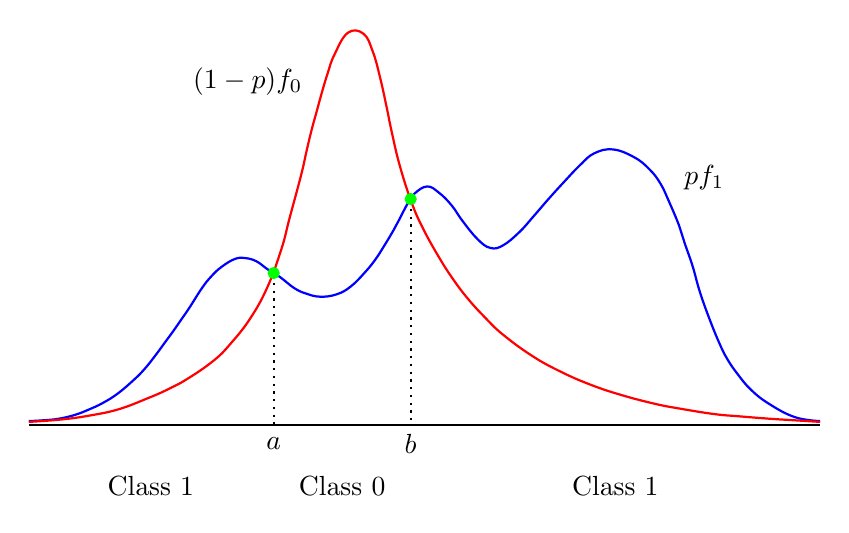
\begin{tikzpicture}
    % p f_1
    \draw [blue, thick] plot[smooth, tension=.7] coordinates {
        (-4.88,-2.08) (-4.70,-2.07) (-4.50,-2.05) (-4.29,-2.00) (-4.11,-1.93)
        (-3.94,-1.85) (-3.75,-1.73) (-3.55,-1.56) (-3.42,-1.43) (-3.29,-1.27)
        (-3.15,-1.08) (-3.04,-0.93) (-2.95,-0.80) (-2.84,-0.64) (-2.68,-0.39)
        (-2.56,-0.24) (-2.43,-0.12) (-2.26,-0.02) (-2.13,-0.01) (-1.99,-0.05)
        (-1.85,-0.15) (-1.69,-0.25)  % first crossing (a)
        (-1.51,-0.39) (-1.36,-0.46) (-1.18,-0.50) (-0.97,-0.47) (-0.79,-0.37)
        (-0.61,-0.19) (-0.48,-0.03) (-0.37, 0.14) (-0.25, 0.34) (-0.18, 0.47)
        (-0.07, 0.68) ( 0.02, 0.81)  % second crossing (b)
        ( 0.18, 0.90) ( 0.33, 0.82) ( 0.49, 0.66) ( 0.63, 0.46) ( 0.82, 0.23)
        ( 0.98, 0.12) ( 1.14, 0.15) ( 1.35, 0.32) ( 1.53, 0.52) ( 1.72, 0.74)
        ( 1.92, 0.96) ( 2.12, 1.17) ( 2.30, 1.32) ( 2.54, 1.37) ( 2.81, 1.27)
        ( 3.00, 1.12) ( 3.14, 0.94) ( 3.25, 0.71) ( 3.38, 0.40) ( 3.45, 0.18)
        ( 3.55,-0.11) ( 3.64,-0.43) ( 3.76,-0.77) ( 3.89,-1.09) ( 3.99,-1.29)
        ( 4.12,-1.48) ( 4.29,-1.68) ( 4.52,-1.86) ( 4.85,-2.03) ( 5.17,-2.08)
    };
    \node at ( 3.70, 1.01) {$pf_{1}$};  % label

    % (1-p) f_0
    \draw [red, thick] plot[smooth, tension=.7] coordinates {
        (-4.88,-2.09) (-4.47,-2.06) (-4.11,-2.01) (-3.74,-1.93) (-3.37,-1.79)
        (-3.12,-1.68) (-2.86,-1.54) (-2.53,-1.31) (-2.32,-1.10) (-2.07,-0.78)
        (-1.85,-0.38) (-1.67, 0.11)  % first crossing (a)
        (-1.57, 0.49) (-1.42, 1.05) (-1.35, 1.36) (-1.29, 1.61) (-1.23, 1.83)
        (-1.15, 2.12) (-1.08, 2.35) (-1.00, 2.57) (-0.83, 2.85) (-0.63, 2.84)
        (-0.51, 2.61) (-0.42, 2.29) (-0.34, 1.93) (-0.27, 1.59)
        (-0.17, 1.17) (-0.02, 0.70)  % second crossing (b)
        ( 0.13, 0.36) ( 0.33, 0.00) ( 0.51,-0.28) ( 0.70,-0.53) ( 0.91,-0.76)
        ( 1.14,-0.98) ( 1.51,-1.25) ( 1.87,-1.45) ( 2.26,-1.62) ( 2.65,-1.75)
        ( 3.07,-1.86) ( 3.38,-1.92) ( 3.82,-1.99) ( 4.15,-2.02) ( 4.53,-2.05)
        ( 4.85,-2.07) ( 5.17,-2.09)
    };
    \node at (-2.10, 2.23) {$(1-p)f_{0}$};  % label

    % first crossing (a)
    \draw [green] (-1.77,-0.20) node (a) {} circle (2pt);  % circle (a)
    \fill [green, thick] (a) circle (2pt);                 % fill circle
    \draw [dotted, thick] (a) -- (-1.77,-2.13);            % dotted line to x-axis
    \node at (-1.77,-2.37) {$a$};                          % label on x-axis

    % second crossing (b)
    \draw [green] (-0.03, 0.74) node (b) {} circle (2pt);  % circle (b)
    \fill [green, thick] (b) circle (2pt);                 % fill circle
    \draw [dotted, thick] (b) -- (-0.03,-2.13);            % dotted line to x-axis
    \node at (-0.03,-2.37) {$b$};                          % label on x-axis

    % x-axis & class labels
    \draw (-4.88,-2.13) -- ( 5.17,-2.13);  % x-axis
    \node at (-3.33,-2.90) {Class 1};      % (-\infty, a)
    \node at (-0.90,-2.90) {Class 0};      % [a, b]
    \node at ( 2.57,-2.90) {Class 1};      % (b, \infty)
\end{tikzpicture}
}
    \caption{%
        Illustration of the Bayes classifier in case the distribution of $X$ is given by a density $f$ and conditional densities $f_0$ and $f_1$ exist. The classifier equals $0$ on the interval $[a, b]$ and $1$ elsewhere.
    }
\end{figure}
If we additionally assume that both classes are equally likely, i.e., $p = 1 - p = 1/2$, the Bayes classifier becomes
\[
    h^*(x) = \begin{cases}
        1, \quad & f_1(x) > f_0(x) \\
        0, \quad & \text{else}
    \end{cases}
\]
and its error is given by
\[
    L^* = \frac{1}{2} \int_{\mathcal{X}} \min(f_1(x), f_0(x)) \dx = \frac{1}{2} \int_{\mathcal{X}} f_1(x) - (f_1(x) - f_0(x))^{+} \dx = \frac{1}{2} - \frac{1}{4} \int_{\mathcal{X}} \abs{f_1(x) - f_0(x)} \dx,
\]
where $g^{+} = \max(g, 0)$ denotes the positive part of a function $g \in \R^{\mathcal{X}}$. This demonstrates that the Bayes error is directly related to the $L^1$-distance between the class densities $f_1$ and $f_0$.
